\chapter{背景}
\label{background}

本章では本研究の背景について述べる.

\section{ネットワーク音楽演奏}
ネットワークを介して複数の演奏者がリアルタイムで演奏を行うことをネットワーク音楽演奏と呼ぶ.
一概にネットワーク音楽演奏と言っても同じローカルネットワークに繋がった小規模なものから,インターネットを介して世界中の演奏者が繋がった大規模なものまで様々なものがある.
また演奏者の数も1対1のデュエットから,オーケストラ規模の多くの人を同時に繋げたシステムまで可能である.
そのうえ近年では音声だけでなく視覚情報を含めた視聴覚体験を提供するネットワーク音楽演奏のシステムも研究されている.

上記の通りネットワーク音楽演奏には様々なものがあるが,いずれも演奏者の音声をリアルタイムで相手に届けることが重要であり,これには主に二種類の方法がある.
音響情報をVoIPアプリケーションなどで送信する方法と,音声情報をMIDIやOSCなどの記号に圧縮し,抽象的なデータとして送信する方法である.

本研究では1対1のインターネットを介したネットワーク音楽演奏を想定し,後者の音声情報をOSCで送信する方法を用いる.

\section{ネットワーク音楽演奏システムの構造}
\label{background:structure}
本研究で用いるネットワーク音楽演奏システムの構図はIorwerthらによる"Playing Together Apart Framework (PTA)"を用いる.PTAフレームワークについては図\ref{fig:structure}に示す.

\begin{figure}[htbp]
  \centering
  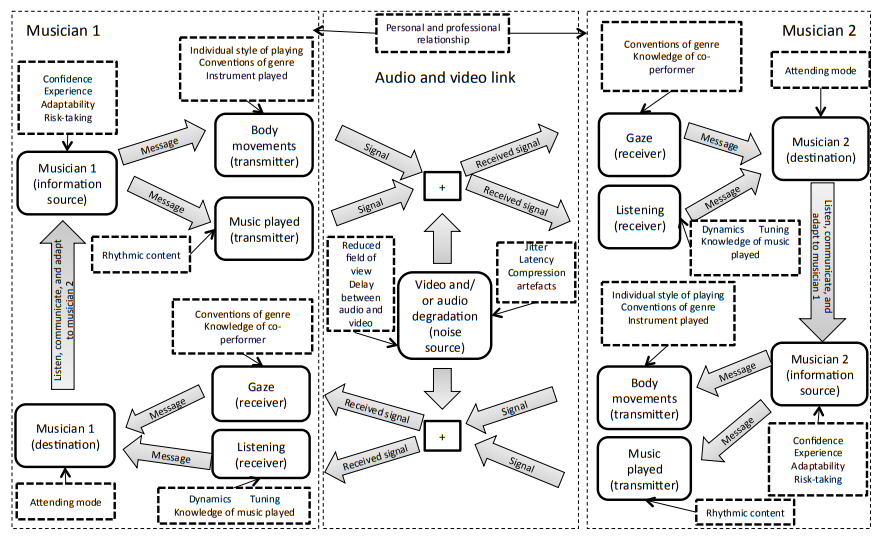
\includegraphics[width=0.8\linewidth]{src/playing_together_apart_framework.png}
  \caption{PTAフレームワーク.\cite{pta}より引用}
  \label{fig:structure}
\end{figure}

TODO: 日本語訳
以上の通り片方の演奏者からもう一方の演奏者に届くまで5つの工程がある.

1. 演奏者の演奏
2. 演奏の発信
3. 情報の圧縮,ネットワークを介した送信
4. 情報の受信,圧縮の解除
5. 演奏の再生

\subsection{OpenSound Control}
OpenSound Control (OSC)は音響情報を記号に圧縮し,抽象的なデータとして送信するためのプロトコルである.本研究ではOSCを用いて音声情報を送信する.
----- OSCの詳細については後述する.

\section{Adaptive Metronome}
BattelloらによるAdaptive Metronome\cite{admet}\cite{admet:experiment}は,演奏者の演奏をリアルタイムで分析し,演奏者の演奏に合わせてメトロノームのテンポを変化させるシステムである.

\begin{figure}[htbp]
  \centering
  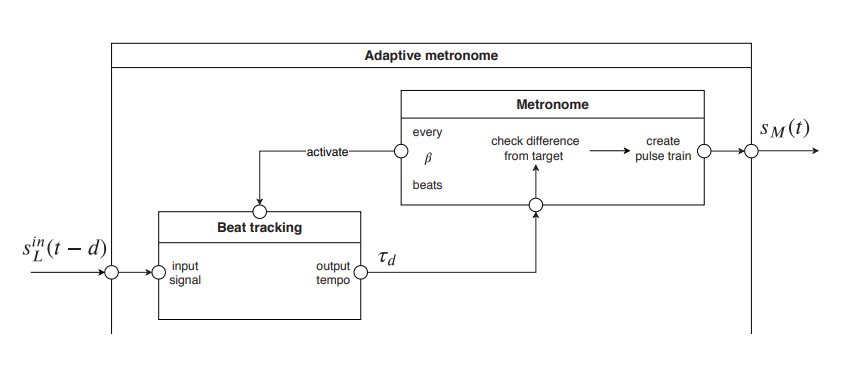
\includegraphics[width=0.8\linewidth]{src/admet.png}
  \caption{Adaptive Metronomeの実験\cite{admet}}
  \label{fig:admet}
\end{figure}

Adaptive Metronomeは親子構造を持っている.
親の演奏者は演奏すると同時にシステムはリアルタイムでその演奏の拍を推定し,子演奏者に音声と拍情報を送信する.
子演奏者のシステムはその情報を受取り,親演奏者の演奏に合わせてメトロノームのテンポを変化させる.
またこのときメトロノームの音は親から子への遅延を考慮して位相をずれして再生される.

こうすることで小演奏者に聞こえるメトロノームは親演奏者の遅延された演奏に関わらず,常に親演奏者の無遅延の演奏に合わせたテンポで再生される.
このシステムを用いた実験では120msの遅延下での演奏を行ったうえでも,被験者は抵抗を感じることなく演奏することができたという結果が得られた.\cite{admet}

\subsection{相互メトロノームの実験}
当初のAdaptive Metronomeの実験では,親演奏者の演奏を子演奏者が聴き,それに合わせて演奏するという形で実験が行われた.
後にBatteloらは親子構造を持たず,相互的にAdaptive Metronomeを聞きあう実験を行った.
実験の結果は現状まだ不十分であるが,このような相互的なシステムでもある程度の効果が得られることが示された.

\subsection{共通テンポの算出}
相互的にAdaptive Metronomeを聞きあう実験では,全体のテンポを決定させる親演奏者がいないため,演奏者同士のテンポと位相が異なる場合がある.
このとき2人の演奏者の状況を踏まえたうえで両方の演奏が同期するような共通のテンポを算出する必要がある.

\section{Tablanet}
Tablanet\cite{tablanet}は,タブラ奏者の演奏をリアルタイムで分析し,演奏者の演奏に合わせてタブラのテンポを変化させるシステムである.

\section{Alexandraki}
Alexandrakiらによる研究\cite{alexandraki:2013}\cite{alexandraki:2014}では,演奏者の演奏をリアルタイムで分析し,事前収録した演奏を実際の演奏に合わせて再生するシステムを提案している.
